
\chapter{Divertimento: un bongo}

\lettrine[lines=2]{C}{uando Cecilia} entró a la oficina de Antonia
encontró una sorpresa sobre su escritorio.

---¿Y eso..?  ---preguntó.

\begin{figure}[ht]
  \centering
  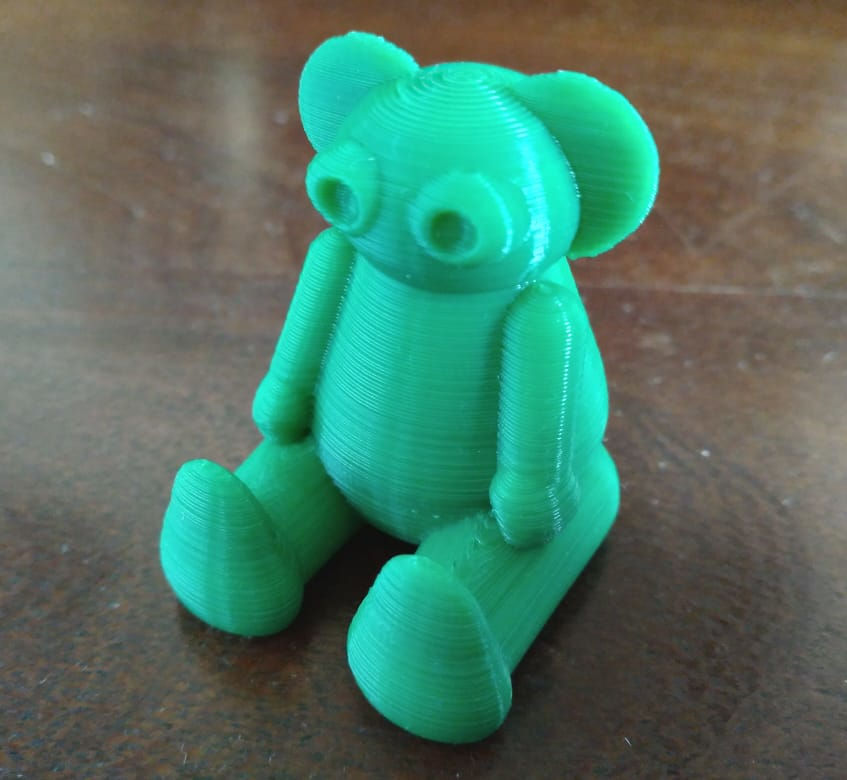
\includegraphics[width=.65\textwidth]{imagenes/bongo2}
  \caption{Un bongo.}
  \label{fig:bongo2}
\end{figure}
  


---Un bongo ---respondió Antonia con naturalidad.

---¿Un bongo? ---preguntó nuevamente Cecilia.

---Sí, un bongo ---reafirmó su amiga con cara de sor\-pre\-sa---. Los
bongos eran personajes del juego `\emph{Dr. Peppers and the
  bongos}'. No me digas que no te acordás...

Cecilia arqueó las cejas demostrando ignorar la existencia de ese
juego.

---Ay, Cecilia; ¡por favor! ---Antonia subrayó su asombro separando
los brazos del cuerpo ostensiblemente---. ¿Dónde estuviste en la
década del '80? \emph{Dr. Peppers and the bongos} fue un juego
revolucionario para su época: exhibió el primer motor 3D de la
historia. Era un tanto rudimentario, es verdad; pero muy
jugable. Además de que como juego era muy divertido.\footnote{Admito
  que la referencia de Antonia al juego \emph{Dr. Peppers and the
    bongos} me toma por sorpresa a mí también. He fatigado Internet en
  busca de mayor información y no he podido arribar a nada concreto,
  salvo unos enlaces rotos a una efímera página de Wikipedia que al
  parecer fuera borrada por manos anónimas. (Nota del Editor)} En fin,
¿te gusta?

Cecilia miró de cerca el bongo. Le pareció bonito y
simpático.

---Sí ---contestó.

---Qué bueno, porque es tuyo ---la mirada de Cecilia debió haber
reflejado su sorpresa, porque Antonia sintió la necesidad de ser más
clara---: Sí; es un regalo.

Cecilia no sabía qué decir: era la primera vez que Antonia le hacía
uno.

---Gracias... ---pudo soltar apenas, tras unos instantes.

\section{\texttt{hull()}}


Cecilia movía suavemente el bongo entre sus manos:

---Antonia, pensé que \openscad{} sólo permitía crear objetos más
bien... `geométricos'. ¿Como obtuviste estas formas tan redondeadas y
suaves? ---quiso decir ``tiernas'', pero no se animó.

---Tengo mis trucos ---deslizó Antonia con un guiño---. El primero es
la transformación \lstinline!hull()!:
    

    \begin{lstlisting}
$fn=100;      
hull() {
 sphere(r=10);
 translate([0,0,30])
   sphere(r=5);
}
    \end{lstlisting}%$

    \begin{figure}[ht]
      \centering
  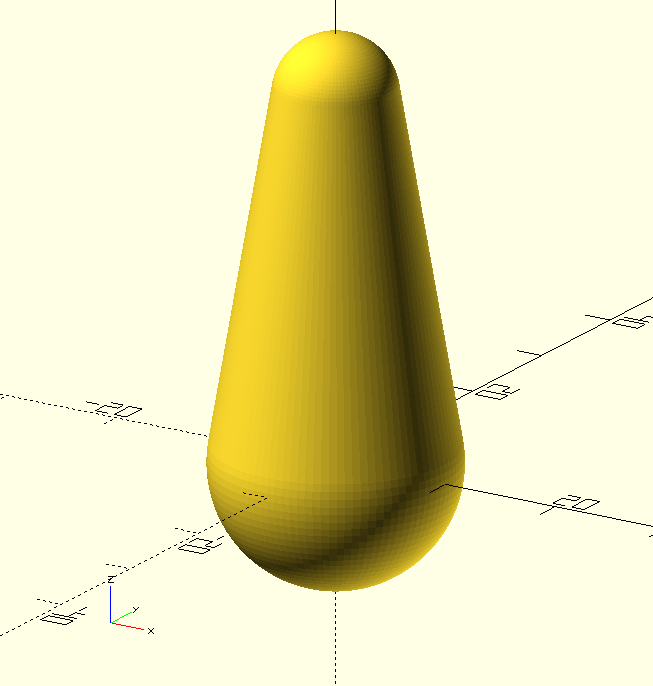
\includegraphics[width=.48\textwidth]{imagenes/hull-1}\hfill
  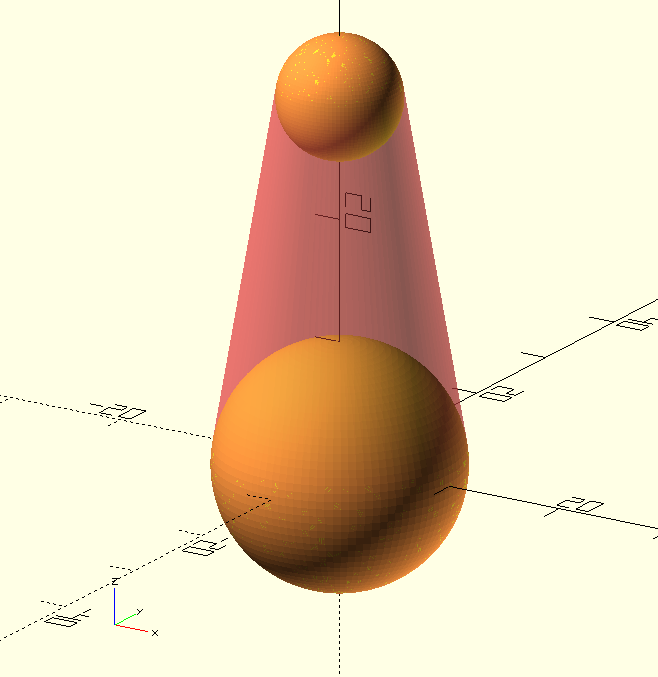
\includegraphics[width=.48\textwidth]{imagenes/hull-2}
  \caption{Antonia ofrece un rápido ejemplo de la operación
  \lstinline!hull()!.}
      \label{fig:hull}
    \end{figure}

    \guillemotright \lstinline!hull()! toma los objetos que le pasás
    entre llaves y crea un nuevo objeto que es su envolvente convexa
    ---Antonia miró fugazmente el techo como buscando algo más
    parecido a una explicación---. Imaginate que rodeas a los objetos
    entre llaves con una suerte de envoltura de goma bien ajustada;
    bueno, eso es lo que hace \lstinline!hull()!.  En la imagen
    izquierda de la figura \ref{fig:hull} te muestro el resultado del
    texto que escribí; a la derecha destaqué artificialmente las dos
    esferas entre llaves, para que se note mejor su estructura.

    Cecilia miraba el monitor con una cara que no inspiraba confianza
    en los poderes explicativos de Antonia.

---A ver con otro ejemplo... ---insistió---. Ahora voy
  a envolver un cubo en la base con un cilindro en la punta:

    \begin{lstlisting}
$fn=100;
hull() {
 cube([30,30,10],center=true);
 translate([0,0,40])
   cylinder(h=5,r=5);
}
    \end{lstlisting}%$

    \begin{figure}[ht]
      \centering
  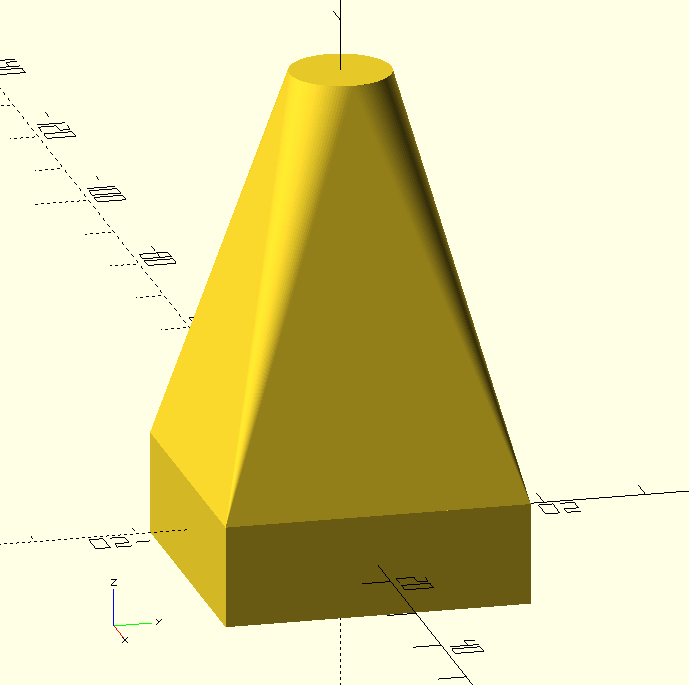
\includegraphics[width=.46\textwidth]{imagenes/hull-3}\hfill
  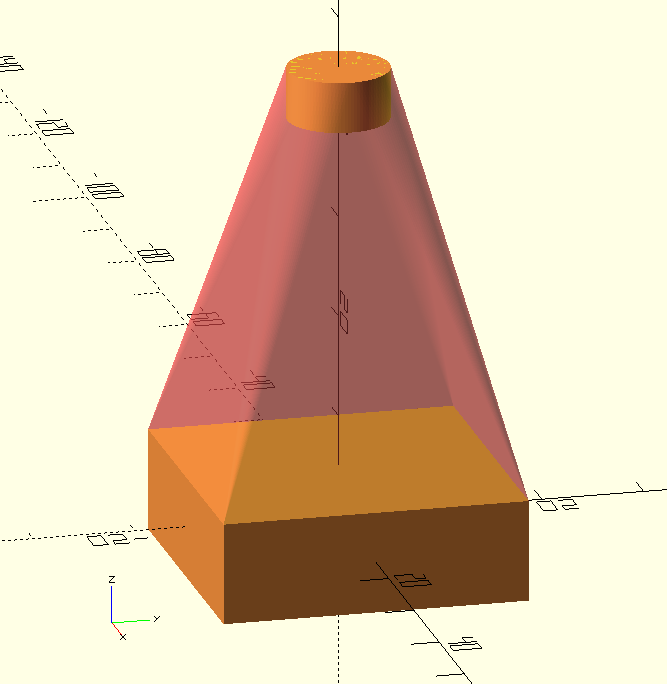
\includegraphics[width=.46\textwidth]{imagenes/hull-4}      
  \caption{Otro ejemplo de \lstinline!hull()!.}
      \label{fig:hull-2}
    \end{figure}


    \guillemotright Acordate de que el objeto producido por
    \lstinline!hull()! es el de la izquierda; el otro lo hice para
    destacar su estructura interna, nomás ---alertó Antonia, y
    continuó---: Con esto, ya podemos escribir el cuerpo del bongo.

    \begin{lstlisting}
$fn=100;
module cuerpo(){
  hull() {
    translate([0,0,3]) sphere (d=12);
    translate([0,0,11.25]) sphere (d=6);
  }
}
cuerpo();
    \end{lstlisting}%$

    \begin{figure}[ht]
      \centering
  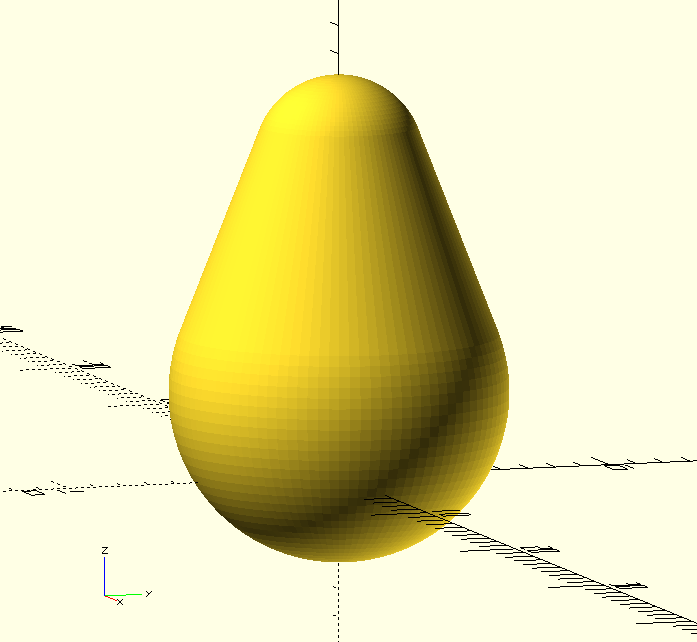
\includegraphics[width=.7\textwidth]{imagenes/cuerpo}      
      \caption{Cuerpo del bongo.}
      \label{fig:cuerpo-bongo}
    \end{figure}


    Cecilia sonrió, no sabemos si porque comprendía cabalmente lo que
    Antonia estaba haciendo o porque el cuerpo del bongo había quedado
    muy lindo.

    ---¿Por qué usaste esos valores? En particular el 11,25?
    ---pre\-gun\-tó.

    ---Ay, Cecilia... ¡porque sí! ---respondió su amiga con una risa
    ligera---. Dale, relajate... no todo tiene que depender de
    cálculos estrechos y rigurosos... pongamos números `a ojito' y ya
    fue...

    Cecilia estaba sorprendida; nunca había visto a Antonia con ese
    desenfado. Pero inmediatamente recordó que desde siempre parecía
    reservarse el privilegio de desconcertarla. Y el bongo había
    quedado realmente bonito, así que decidió seguirle el juego.

    ---Fijate ---explicó Antonia---: usé dos esferas y las envolví en
    un \lstinline!hull()!. En la figura \ref{fig:cuerpo-transparente}
    te destaco, una vez más, la estructura interna.

\begin{figure}[ht]
  \centering
  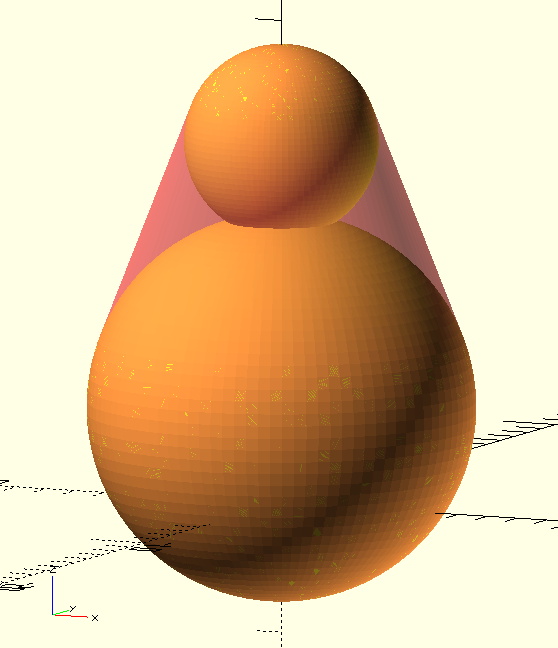
\includegraphics[width=.5\textwidth]{imagenes/cuerpo-transparente}
  \caption{Estructura del cuerpo del bongo, rodeada por el
    \lstinline!hull()!.}
  \label{fig:cuerpo-transparente}
\end{figure}
  


\section{\texttt{scale()}}


\guillemotright Ahora creo que es el turno de la cabeza. Como sabemos, los
  bongos tienen una cabeza más ancha que alta. Para lograrla usaremos
  lo transformación \lstinline!scale()!.

\begin{figure}[ht]
  \begin{minipage}[]{.5\textwidth}
    \begin{lstlisting}
module cabeza() {
  translate([0,0,12.75])
    scale([1,1,.8]) 
      sphere(d=9);
}

cabeza();
  \end{lstlisting}
  \end{minipage}\hfill
  \begin{minipage}[]{.45\textwidth}
      \centering
      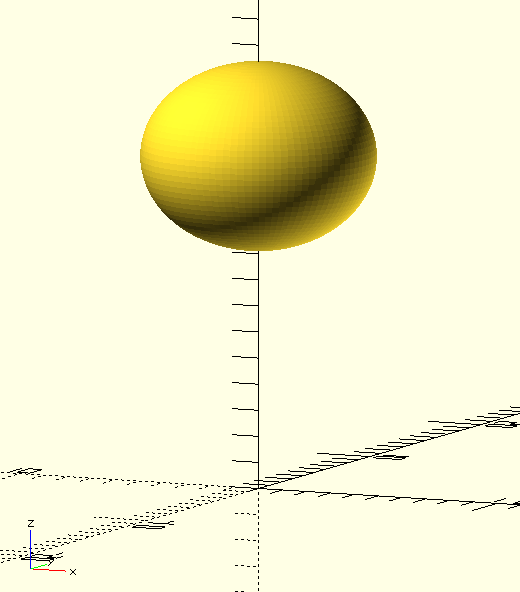
\includegraphics[width=.7\textwidth]{imagenes/cabeza-1}
    \end{minipage}
    \caption{Antonia usa la transformación \lstinline!scale! para dar
      forma a la cabeza del bongo.}
    \label{fig:cabeza-1}
  \end{figure}
  
  \guillemotright Como su nombre sugiere, \lstinline!scale()! realiza
  un escalado del objeto al cual se aplica en cada uno de sus tres
  ejes. En el caso de la cabeza del bongo, como podés ver en la figura
  \ref{fig:cabeza-1}, toma la esfera y deja igual su tamaño en
  \coord{X} e \coord{Y}, pero multiplica su longitud en \coord{Z} por
  0,8. Debido a eso, la `aplasta' ---Antonia replicó el efecto
  acercando las palmas de sus manos dispuestas horizontalmente, una
  encima de la otra; al parecer, pertenecía al grupo de docentes que
  consideran que mover las manos equivale a ex\-pli\-\mbox{car---.} El
  escalado te permite, por ejemplo, realizar cilindros de base
  ovalada, o `pastillas'; fijate la figura \ref{fig:pastillas}.

    \begin{figure}[ht]
  \begin{minipage}[]{.5\textwidth}
    \begin{lstlisting}
scale([1,.5,1])
  cylinder(r=10,h=30);
  
translate([40,0,15])
  scale([2,1,.5])
    sphere(r=10);
  \end{lstlisting}
  \end{minipage}\hfill
  \begin{minipage}[]{.45\textwidth}
      \centering
      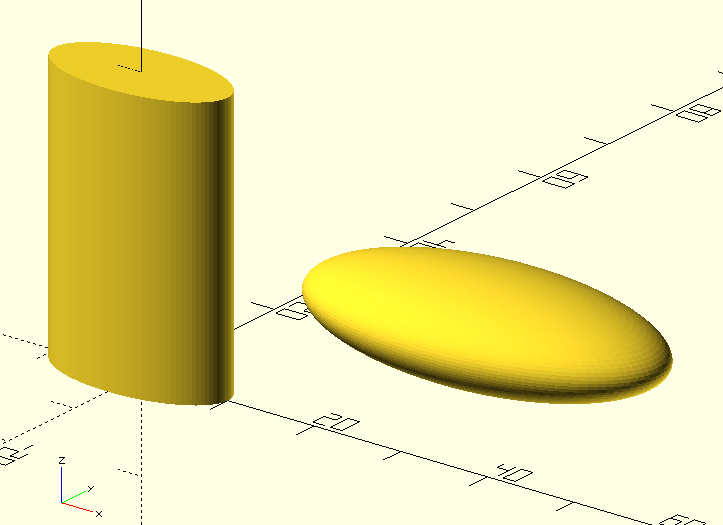
\includegraphics[width=.9\textwidth]{imagenes/scale}
    \end{minipage}
    \caption{Antonia ofrece dos ejemplos más de la transformación
      \lstinline!scale!.}
    \label{fig:pastillas}
  \end{figure}

  \guillemotright La `pastilla', como verás, fue alargada dos veces en el eje
  \coord{X} y achicada a la mitad en el \coord{Z} ---desarrolló
  Antonia, y agregó---: El escalado me resultó útil para escribir
  también el ojo del bongo.

        \begin{center}
  \begin{minipage}[]{.64\textwidth}
    \begin{lstlisting}
module ojo() {
 translate([1.8,-3.25,13.35]){
  difference() {    
   // globo ocular
   scale([1.3,1,1]) 
    sphere(d=3);
   // iris 
   translate([0.25,-1.56,0]) 
    sphere(d=1.8);
   }
  }
}
ojo();
\end{lstlisting}
  \end{minipage}\hfill
  \begin{minipage}[]{.35\textwidth}
      \centering
      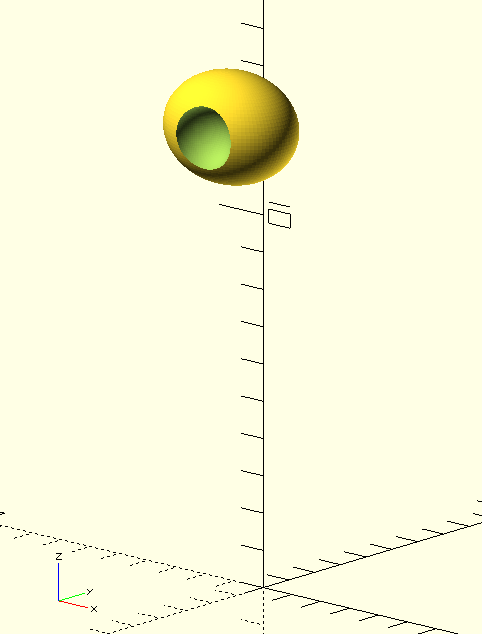
\includegraphics[width=\textwidth]{imagenes/ojo}
    \end{minipage}
  \end{center}

  \guillemotright Para terminar con la cabeza nos faltan las orejas
  que caracterizaron, desde tiempos inmemoriales, a los bongos
  ---Antonia tecleó con rapidez, mientras ladeaba ligeramente la
  cabeza como quien comprueba el efecto de las pinceladas sobre un
  lienzo:

          \begin{center}
  \begin{minipage}[]{.6\textwidth}
    \begin{lstlisting}
module oreja() {
 translate([3.6,0,13.95])
  scale([1,.2,1])
   sphere(d=6);
}
oreja();
\end{lstlisting}
  \end{minipage}\hfill
  \begin{minipage}[]{.4\textwidth}
      \centering
      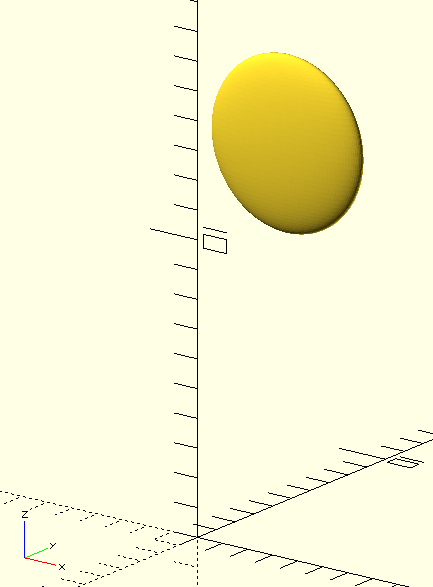
\includegraphics[width=.7\textwidth]{imagenes/oreja}
    \end{minipage}
  \end{center}

  ---A ver cómo está quedando... ---intervino Cecilia, que ya tenía
  ganas de escribir.

  \begin{figure}[ht]
      \begin{minipage}[]{.5\textwidth}
\begin{lstlisting}
cuerpo();
cabeza();
ojo();
oreja();
\end{lstlisting}
\end{minipage}
  \begin{minipage}[]{.4\textwidth}
  \centering
  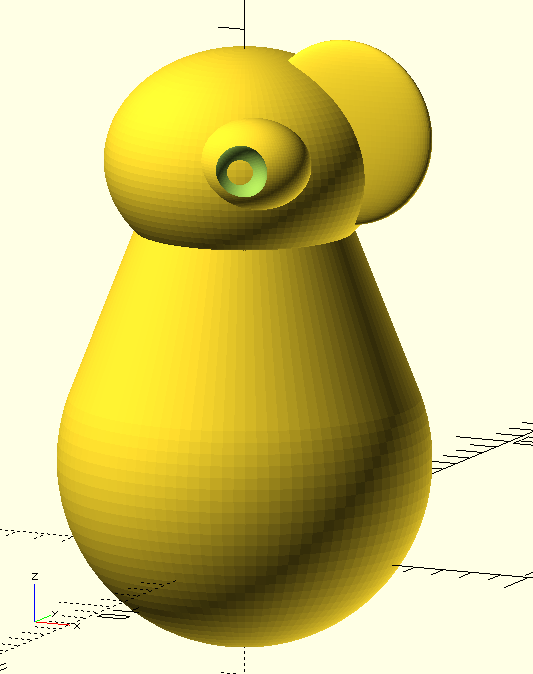
\includegraphics[width=\textwidth]{imagenes/bongo-a-medias}
\end{minipage}
\caption{Bongo a medias.}
  \label{fig:bongo-a-medias}
\end{figure}


---¡Qué lindo! ---exclamó Cecilia ante la figura
\ref{fig:bongo-a-medias}---. Encima parte de la cabeza sobresale del iris
y queda como una pupila... Voy a repetir ojo y oreja trasladándolos la
distancia adecuada.
    
Antonia la detuvo, guiñando un ojo:

---Hay una manera mejor de repetir objetos simétricamente; te sugiero
que sigamos con el brazo y la pierna izquierdos, y después te cuento
cómo replicar todo del lado derecho del bongo.

A Cecilia le pareció natural que \openscad{} contara con una
transformación que diera cuenta de los modelos que presentan simetría
bilateral, así que decidió confiar en Antonia.

---El resto de los miembros del bongo no respresenta ninguna
herramienta nueva; se trata de escribir, nomás ---a\-de\-lan\-tó
Antonia.

    \begin{lstlisting}
module brazo () {
 rotate([0,0,-20])
  translate([4.2,0,9])   
   rotate([20,159,0]) {
    // brazo
    hull () {
     sphere(d=3);
     translate([0,0,6])
       sphere (d=2.4);
     }
     // mano
     translate([-0.12,0,6])
      scale([.69,1,1]) 
       sphere (d=3.6);
    }      
}  
brazo();
\end{lstlisting}

\begin{figure}[ht]
  \centering
    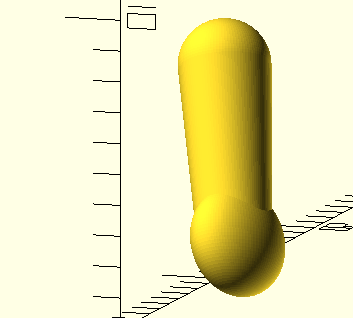
\includegraphics[width=.35\textwidth]{imagenes/brazo}
  \caption{Brazo del Bongo}
  \label{fig:brazo}
\end{figure}

 \begin{lstlisting}
module pierna(){
 translate([4.2,0,0])
  rotate([90,0,0]){
   // pierna
   hull(){
    sphere(d=6);
    translate([0,0,8.4])
     sphere(d=4.8);
     }
   // pie
   hull(){
    translate([0,0,9.6]) 
     scale([1,1,.6])
      sphere(d=6);
    translate([0,3.6,9.6]) 
      scale([1,1,.4])
     sphere(d=3.6);
     } 
  }
}
pierna();
 \end{lstlisting}

\begin{figure}[ht]
  \centering
      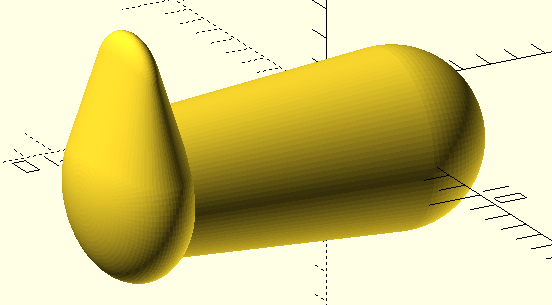
\includegraphics[width=.35\textwidth]{imagenes/pierna}
  \caption{Pierna del Bongo}
  \label{fig:pierna}
\end{figure}


\guillemotright Vamos a ver todo junto ---propuso Antonia, mientras
producía la figura \ref{fig:medio-bongo}.

  \begin{figure}[ht]
  \begin{minipage}[]{.4\textwidth}
    \begin{lstlisting}
cuerpo();
cabeza();
ojo();
oreja();
brazo();
pierna();
\end{lstlisting}
\end{minipage}
\begin{minipage}[]{.45\textwidth}
  \centering
  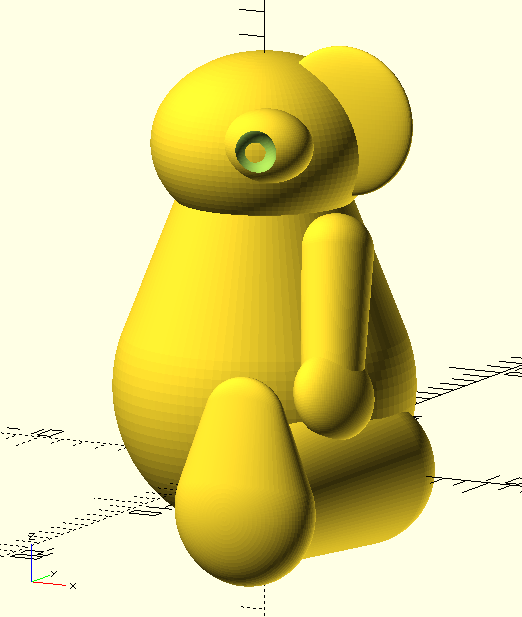
\includegraphics[width=\textwidth]{imagenes/medio-bongo}
\end{minipage}
\caption{Medio bongo.}
  \label{fig:medio-bongo}
\end{figure}


\section{\texttt{mirror()}}


---Lindo, ¿no? ---Antonia buscó la aprobación de su a\-mi\-ga---. Ahora
debemos `espejar' ojo, oreja, brazo y pierna. Pues bien, resulta que
\openscad{} cuenta con una transformación que justamente realiza esa
operación ---añadió, mientras escribía el ejemplo de la figura
\ref{fig:bongo-casi-entero}.

  \begin{figure}[ht]
 \begin{minipage}[]{.4\textwidth}
   \begin{lstlisting}
cuerpo();
cabeza();
ojo();
oreja();
brazo();
pierna();
mirror([1,0,0]){
  ojo();
  oreja();
  brazo();
  pierna();
}
\end{lstlisting}
  \end{minipage}\hfill
  \begin{minipage}[]{.6\textwidth}
    \centering
%\centerline {
      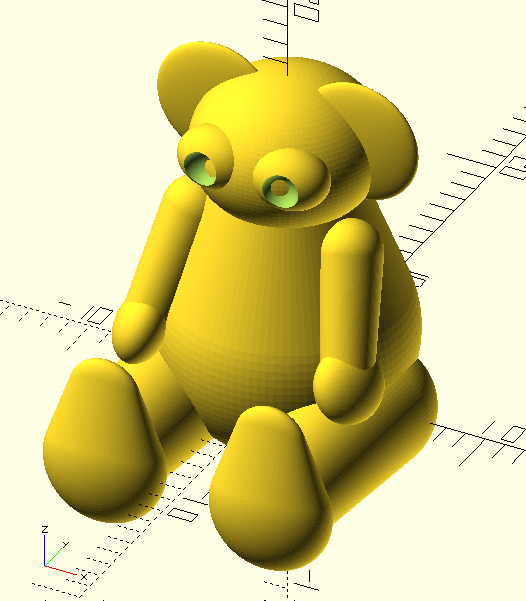
\includegraphics[width=\textwidth]{imagenes/bongo-casi-entero}
    \end{minipage}
    \caption{Antonia replica ojo, oreja, brazo y pierna del bongo
      mediante la transformación \lstinline!mirror()!.}
  \label{fig:bongo-casi-entero}
\end{figure}


\guillemotright \lstinline!mirror()! copia especularmente (y
espectacularmente) ---An\-to\-nia era famosa en todo Harvard por sus
chistes malos y ñoños--- los objetos a los que se aplica (si son más
de uno, deben colocarse entre llaves, como con cualquier otra
transformación). Para decidir cuál es el plano del `espejo', debemos
indicar entre paréntesis un vector cualquiera que sea perpendicular al
mismo; mirá el ejemplo de la figura \ref{fig:mirror-1}.

   \begin{figure}[ht]  
\begin{minipage}[]{.49\textwidth}     
   \begin{lstlisting}
// esfera original     
translate([10,0,0])
 color("red")
  sphere(r=1);
// espeja espejada 
mirror([6,0,0])
 translate([10,0,0])
  color("blue")
   sphere(r=1);
   \end{lstlisting}
 \end{minipage}
\begin{minipage}[]{.5\textwidth}     
 \centering
 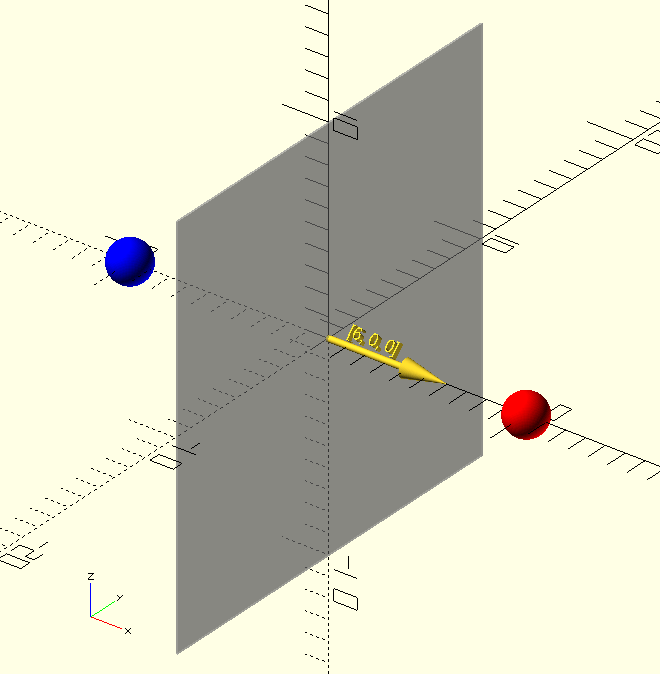
\includegraphics[width=.9\textwidth]{imagenes/mirror-1}
\end{minipage}
\caption{Antonia ofrece un ejemplo de la transformación
        \lstinline!mirror()!.}
     \label{fig:mirror-1}
   \end{figure}
     

  
   \guillemotright En las líneas 2 a 4 escribí una esfera roja, que
   luego copié en las líneas 7 a 9, salvo que de color azul ---explicó
   Antonia, aunque Cecilia era muy capaz de verlo por sí misma---.  En
   la línea 6 antepuse a la segunda esfera la transformación
   \lstinline!mirror([6,0,0])!. La función del vector
   \lstinline![6,0,0]! es definir el plano que indiqué en gris
   (artificialmente, sólo a fines de que se notara). Y este plano es
   el que funciona de `espejo' para reflejar la esfera y ubicarla
   donde está, en lugar de superponerla a la roja.

   ---¿Y por qué aparece el vector? ---cuestionó Cecilia.

   ---¡Ah! Es verdad; también lo coloqué artificialmente, para que se
   notara. \lstinline!mirror()! no dibuja el vector ---agregó
   An\-to\-\mbox{nia---.} La magnitud del vector tampoco es
   importante, sino sólo su dirección: el resultado sería exactamente
   el mismo si hubiéramos usado \lstinline!mirror([1,0,0])!; el
   problema sería que mi vector artificial y pictórico sería diminuto
   y no se vería. El vector puede apuntar en cualquier dirección, por
   supuesto; el plano `reflectante' será siempre el perpendicular al
   mismo.

   Antonia escribió otro ejemplo para Cecilia, quien no estaba segura
   de entender del todo. Se propuso escribir luego otros ejemplos por
   sí misma para terminar de aprehender esta nueva transformación.

   \begin{figure}[ht]
\begin{minipage}[]{.49\textwidth}     
   \begin{lstlisting}
// esfera original     
translate([10,0,0])
 color("red")
  sphere(r=1);
// espeja espejada 
mirror([6,6,0])
 translate([10,0,0])
  color("blue")
   sphere(r=1);
   \end{lstlisting}
 \end{minipage}
 \begin{minipage}[]{.5\textwidth}
   \centering
   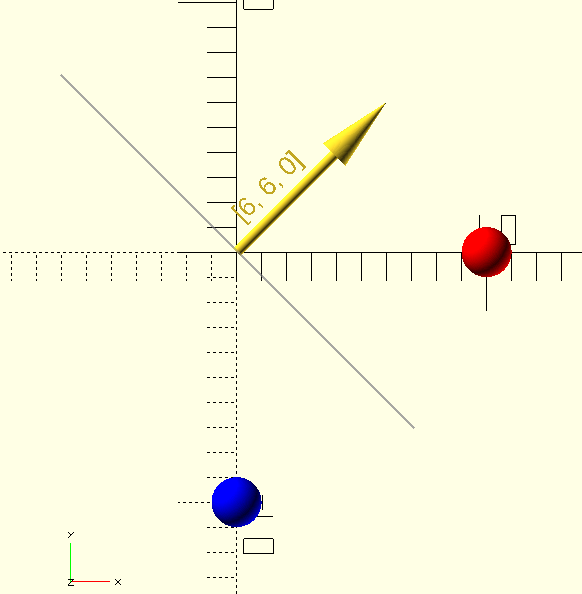
\includegraphics[width=1\textwidth]{imagenes/mirror-2}
 \end{minipage}
 \caption{Otro ejemplo de \lstinline!mirror()!.}
     \label{fig:mirror-2}
   \end{figure}

    \section{\texttt{union()}}

  
    ---Ahora bien, para imprimir el bongo debemos darle una base
    plana. A mí me resultó natural restar un cubo debajo
    ---pro\-pu\-so Antonia.

%           \begin{center}
% \begin{minipage}[]{.6\textwidth}
   \begin{lstlisting}
module bongo(){  
 difference(){
  union(){
   cuerpo();
   cabeza();
   brazo();
   pierna();
   ojo();
   oreja();
   mirror([1,0,0]){
    brazo();
    pierna();
    ojo();
    oreja();
   }
  }
  translate([0,0,-7.7])
     cube ([24,24,12],center=true);
 }
}
bongo();
\end{lstlisting}

\begin{figure}[ht]
  \centering
  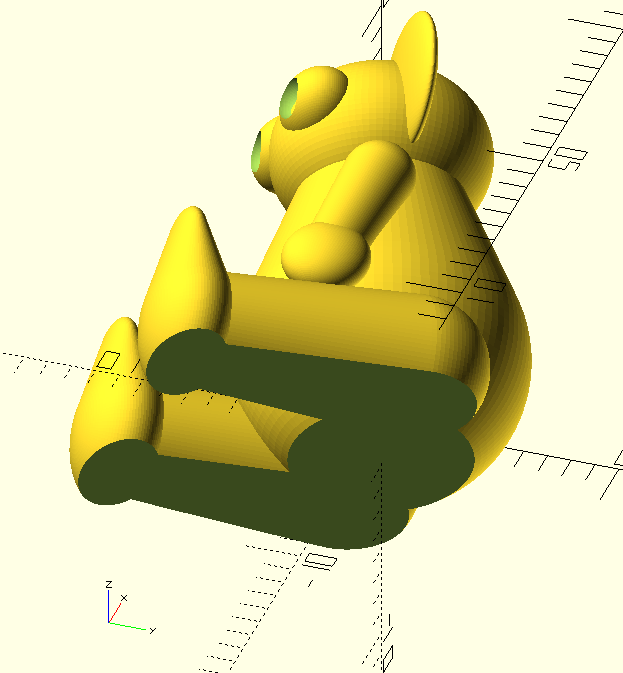
\includegraphics[width=.55\textwidth]{imagenes/bongo-base}  
  \caption{Base del bongo.}
  \label{fig:bongo-base}
\end{figure}


\guillemotright Para ello tuve que usar la transformación
\lstinline!union()!. Bueno, en realidad, no `transforma' nada: une los
objetos que recibe entre llaves como uno solo. Debí usarlo porque yo
quiero que \lstinline!difference()! reste el cubo de las líneas 17 y
18 a \emph{todo} lo anterior. Es decir, desde el punto de vista de
\lstinline!difference()!, el objeto minuendo es el que resulta de
\lstinline!union()!, que dentro de sí abarca a los objetos de las
líneas 4 a 14, y el único cuerpo sustraendo resulta ser el cubo final.

Ambas amigas contemplaban satisfechas el monitor, cuando Antonia se
irguió de golpe en su silla, quizá sobreactuando un poco la alarma:

---¡Oh, no! ¡Por poco me olvido! Un bongo no es un bongo sin rabito:

  
%           \begin{center}
% \begin{minipage}[]{.6\textwidth}
  \begin{lstlisting}
module rabito(){
 translate([0,4.8,-0.3])
  scale([1.2,1.2,1.2])
   sphere(d=3);
}    
bongo();

\end{lstlisting}


\begin{figure}[ht]
  \centering
  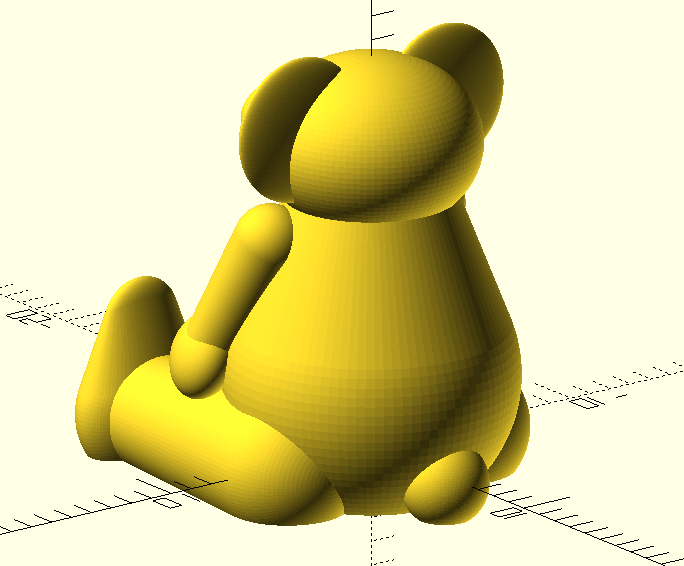
\includegraphics[width=.7\textwidth]{imagenes/bongo-con-rabito}
  \caption{Bongo completo, con todo y rabito.}
  \label{fig:bongo-con-rabito}
\end{figure}

\section{Módulos dentro de módulos}

Antonia aún no parecía satisfecha del todo:

---Supongamos que quisiéramos crear otro muñeco. Es razonable pensar
que debería tener sus propios ojos, cabeza, brazos, piernas, orejas y,
tal vez, incluso un rabito. Pero en ese caso deberíamos bautizar sus
módulos con nombres que no colisionen con los del bongo: algo como
\lstinline!cabeza_vaquita!, por ejemplo.

Cecilia no veía ningún problema en ello, pero tampoco creyó oportuno
disentir al menos hasta ver adónde quería llegar su amiga.

---Creo que los módulos que definen los miembros de los respectivos
muñecos deberían pertenecer unívocamente a los mismos
---ar\-gu\-men\-tó Antonia---. Después de todo, ¿dónde más se puede
usar la oreja de un bongo que no sea en la cabeza de un bongo..?

\guillemotright Por lo tanto, lo que podemos hacer es aprovechar la
posibilidad que nos brinda \openscad{} de escribir módulos dentro de
módulos:

\begin{lstlisting}  
module bongo(){
  module cuerpo(){
    [...]
  }
  module cabeza(){
    [...]
  }
  module brazo(){
    [...]
  }
  [...]    
  difference(){
    union(){
     cuerpo();
     cabeza();
     [...]    
    }
    translate([0,0,-7.7])
      cube ([24,24,12],center=true);
  }
}
\end{lstlisting}

\guillemotright De esta forma, los módulos \texttt{cuerpo},
\texttt{cabeza}, etc., no pueden ser invocados ni aludidos desde fuera
del módulo \texttt{bongo}, por lo que ningún conflicto causarán con
otras extremidades de otros eventuales muñecos.

Cecilia no pudo negar que, al menos como posibilidad, resultaba
interesante.

  

% %%% Local Variables:
% %%% mode: latex
% %%% TeX-master: "../libro"
% %%% End:
